\title{ Correlated mutations and distance correlations to predict aminoacid interactions  \thanks{ Introduction to Python $\&$ Structural Bioinformatics - Master Science in Bioinformatics for Health Sciences at Universitat Pompeu Fabra. This work has been supervised by Javier Garcia and Baldo Oliva}}
\author{Fernando Pozo Ocampo  $\&$ Marcos Camara Donoso}
\date{\today}

\documentclass[12pt]{article}
\usepackage{amsfonts}
\usepackage{amssymb}
\usepackage{amsthm}
\usepackage{hyperref}
\newtheorem{theorem}{Theorem}
\usepackage{mathtools}
\usepackage{enumerate}
\usepackage[a4paper, margin=2.5cm]{geometry}
\usepackage{tikz}
%\usepackage{tikz}
\usetikzlibrary{decorations.markings,arrows}
\usepackage{pgfkeys}
\usepackage{natbib}
\bibliographystyle{nature}
\usepackage{graphicx}
\usepackage{listings}
\usepackage{xcolor}
\lstset{basicstyle=\footnotesize,
  showstringspaces=false,
  commentstyle=\color{orange},
  keywordstyle=\color{blue},
  stringstyle=\color{purple}
}
\usepackage{subfig}


\begin{document}
\maketitle

\begin{abstract}
In this report we describe \textit{CMDC.py}: a software that calculates correlated mutations (CM), which plays a crucial role in molecular evolutionary proccess alongside conservation, and distances correlation in order to predict aminoacid interactions. Since the asumption that correlated mutations are frequently observed among spatially closed residues, correlated mutation analysis (CMA) has been used to predict intra residue contacts (it has been well defined what can be a contact or interaction between residues) from multiple sequence alignment (MSA). From this alignment, it extracts the mutual information (MI), an information theory measure, that has been extensively employed and modified to identify residues within a protein that also are in contact. It relates a normalized value of MI with this mutations and consequently predicts contacts between residues. Finally it substracts a normalized coevolutionary pattern similarity (NCPS) from the normalized Z-scores values of MI in order to remove the noise of the columns and present our results in several plots.
\end{abstract}
\clearpage
\tableofcontents
\clearpage
\section{Introduction}
\subsection{Correlated mutations and distance correlations. A computational method to predict aminoacid interactions}
The structure of a simple protein is one of the most meaningful information carriers in molecular biology. Several well known laboratory experimental methods are used to identify the three-dimensional structure of a protein. These are, however, still expensive and time-consuming. Therefore, several computational methods have been developed, from more than 20 years to now, to predict residue contacts from primary aminoacid sequence and then be able to realise what are the real interactions between aminoacids.\\ 

Correlated mutations (CM) betweeen columns of a multiple sequence alignment (MSA) has been described for protein sequence since many years. First hypothesis of the underlying biological event was, that an unfavorable aminoacid change in a structural contact site may go without negative consequences if its direct binging partner is simultaneously mutated in such a way that the original interaction is rescued, performing as a compensatory mutation\cite{Kowarsch2010}. \\

Analysis of such correlated mutations has been employed for the identification of residue contacts pairs within or even between different protein chains. First approaches to detect co-evolving residues in a MSA was proposed by Göbel and Valencia in 1994\cite{Gobel1994}. From then, another methods have been described and evaluated with respect to their potential of predict residue-residue contacts \cite{Vicatos2005}.\\

However, accuracy of every different methods have supposed a big frontier in this computational approach. Most of studies hardly have shown that prediction accuracies for structural contacts exceed 20-25\%, and loggically it limites the future application of this method to structural prediction in another in silico approaches like \textit{ab initio} structure prediction. Furthermore, it is also relevant to say that there is one new single reference in the bibliography in which with an ultra deep-learning model gets high accuracies in this process, being only effective with some proteins with a very large number of sequence homologs\cite{Wang2016}.\\

Otherwise, it is neccesary to describe in a proper way how can it measure contacts between aminoacids. Two residues are in contact if they are at a lower distance than a distance threshold one to the other. Thus, it can be analyzed by varios distances like $C_{\alpha}$ - $C_{\alpha}$, $C_{\beta}$ - $C_{\beta}$, or minimal distances between the heavy atoms of the side chain of the two residues. It is common to apply a distance value threshold to 8 \r{A} to the $C_{\alpha}$ distances. However, this threshold can fluctuate between 4 and 20 \r{A}\cite{Hunter2007}.\\

In this report, we are going to present below how has been developed our workflow, which takes some of the most common methods in residue contacts prediction in order to well stablished a hard work of several year and trying to get a gold standard way to obtain better results. 
\clearpage
\section{Methods. \textit{CMDC.py} step by step}
\subsection{Steps in aminoacids interaction prediction based on correlated mutations and distance correlations.}
The steps to perform this approach were the following below: 
\begin{enumerate} [i]
\item Performing a BLAST alignment against the FASTA sequence of the protein given in the input, filtering by genus \cite{Sato2003} every sequence obtained in order to create a real correlation in your subsequent analysis. Nr database is recomended due to redundancy reduction\cite{Jeong2012}
\item Multiple Sequence Alignment construction of the complete sequences before (loggically, your reference is included). Clustalomega, Clustalw, Muscle and T-Coffee are available because of looking for the best alignment.
\item Optimize your Multiple Sequence Alignment output for the following calculous of Mutual Information. Sequences with gaps are removed before the joint probability estimation.
\item Mutual Information between pair of residues is calculated applying a correction called Normalized Coevolutionary Pattern Similarity (NCPS)\cite{Lee2009}.
\item Set the right distances between atoms and define what is a contact between $C_{\alpha}$ and $C_{\beta}$ in the program, in order to check if your correlation is reliable.
\item Accuracy computation of your method comparing real and predicted contacts.
\item Plotting the results: 
	\begin{itemize}
		\item Accuracy estimation comparing number of predicted contacts setting the correlation cutoff and the analysis of the precision.
		\item Scatter plot of distance correlation between atoms.
		\item Heatmap between the distances.
		\item Matrix with the predicted contacts exceeding a given threshold over the matrix of mutual information values.
		\item Classical contact map plots which is also useful to identify patterns into a concrete protein.
	\end{itemize}
\end{enumerate}

\subsection{Our workflow}
\textit{CMDC.py} workflow for detecting correlated mutations and distance correlations 
is summarized in the following figure:

\vspace{1cm}
\begin{figure}[h]
\centering
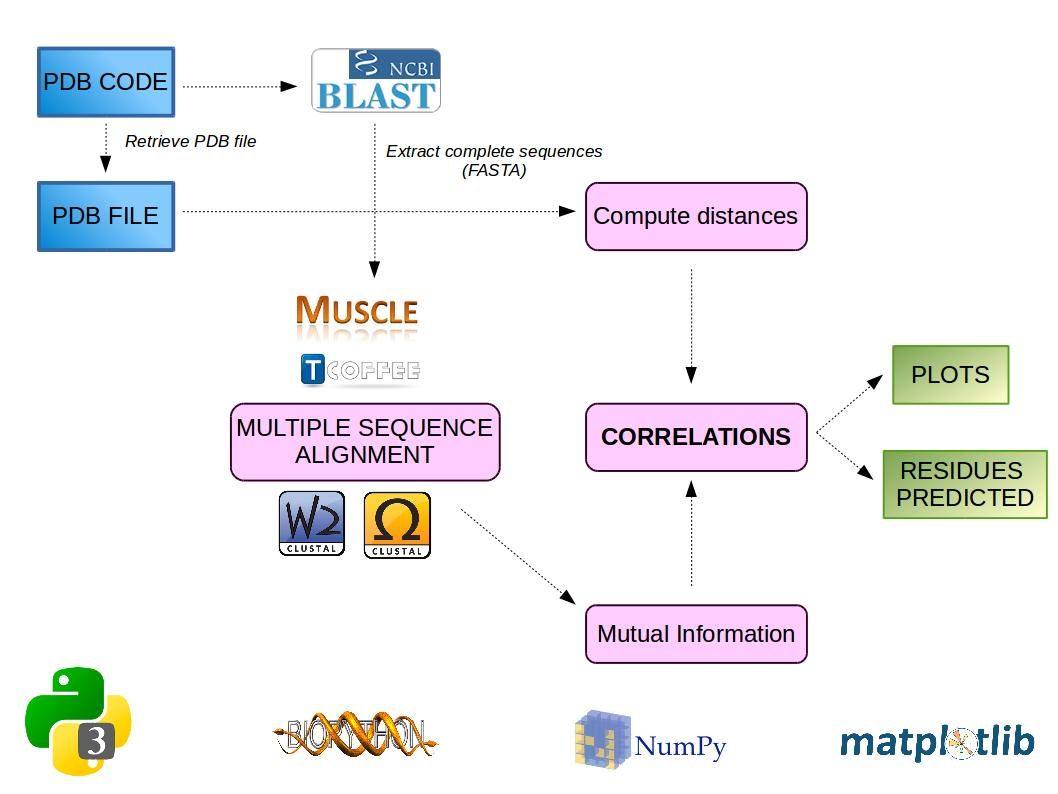
\includegraphics[scale=0.45]{workflow}
\caption{Entire Workflow for CMDC.py}
\label{fig:workflow}
\end{figure}

As seen in the figure \ref{fig:workflow}, user can introduce either a pdb file or a pdb code. If user introduce a pdb code, then the software retrieve the file entry from nr, pdb or swissprot, giving the possibility to choose and always taking into account that internet connection was available. The following step will be the calculous of distance between residues. The results could fluctuate depends of the option selected ($C_{\alpha}$-$C_{\alpha}$, $C_{\beta}$-$C_{\beta}$ or minimum distance) \\
During the execution of the program, after BLAST alignment and the MSA with the MSA method selected, user will check in his directory how FASTA aligned file and BLAST output are obtained. User can select how many sequences hits desire in his BLAST alignment output and whether genus filter is added. Also an standard output is joined if user wants to check every step of the analysis.\\
Consequently, when that MSA is performed, \textit{CMDC.py} calculates frequencies, joint frequencies, entropies and joint entropies in order to obtain the mutual information values. The whole dataset is structured in a matrix of values and is compared by a matrix of hits. Normalized coevolutionary
pattern similarityis substracted from the mutual information values and finally getting more reliable results due to noise reduction.\\ Before running that counts, MSA aligned FASTA file is edited to remove columns with gaps as we explain in last section. An aditional option was added to the user if he does not want to use this correction. \\
Finally, the program gives a file with the positions of residue contacts and plots commented before saved in a file.\\
It has said that two of the modules, \textit{distances.py} and \textit{mi.py} could be also executed standalone. If anybody wants to run only this standalone modules, he can check the documentation with of usage typing the help usage in command line.

\subsubsection{USAGE: Checking dependencies}
First, before starting the execution of the program user have to check if the required packages are installed. User must install \textbf{numpy}\cite{VanderWalt2011}, \textbf{BioPython}\cite{Cock2009}, \textbf{matplotlib}\cite{Hunter2007}, \textbf{pylab} and \textbf{disutils} in order to run properly our program. \textit{sys}, \textit{argparse}, \textit{os}, \textit{urllib}, \textit{ftplib}, \textit{copy} and \textit{math} are also used. Main directory of the execution file also has to contain the other non-standard modules: extract\_sequences.py, distances.py and mi.py. Fast execution, right usage and three execution examples are explained below.\\
On the other hand, you have to check if one MSA software is installed locally in your computer. ClustalW, T-Coffee, ClustalO and Muscle are the options.

\subsubsection{USAGE: Easy, fast and automatic execution and output}
First of all, user can execute the program in a bash executable. This scripts gives the option to compare the results of three differents outputs of the program with three different proteins and options selected. Also he can change the command line order as we will explain in the following sections.

\begin{lstlisting}[language=bash]
$ chmod u+x run.sh
$ ./run.sh
\end{lstlisting}
After approximately 10 minutes, you will find in your directory:
\begin{lstlisting}[language=bash]
$ ls
CMDCresults run.sh README.md CMDC.py distances.py mi.py extract_sequences.py 
$ cd CMDCresults
$ ls
CMDC_01Example_results CMDC_02Example_results CMDC_03Example_results 
$ cd CMDC_01Example_results
$ ls
my_scripts outputs pdb5cyt.ent plots std.sys
\end{lstlisting}
	

\subsubsection{USAGE: General usage}
General usage of the software is:
\begin{lstlisting}[language=python]
$ python3 CMDC.py (pdb code)
\end{lstlisting}

Arguments stablished by default are not typed above. Complete list of argument options (sorted list):
\begin{itemize}
		\item \textbf{pdb code} (mandatory)
		\item -atom (optional) OPTIONS: CA, CB, min  DESCRIPTION: Residues atom to calculate distances: Alpha carbon, beta carbon and min (minimum distance between atom pairs from each aminoacid). DEFAULT: min
		\item -CA (optional) OPTIONS: integer DESCRIPTION: Threshold for alpha carbon atoms in \r{A}. DEFAULT: 8
		\item -CB (optional) OPTIONS: integer DESCRIPTION: Threshold for beta carbon atoms in \r{A}. DEFAULT: 8
		\item -min (optional) OPTIONS: integer DESCRIPTION: Set the minimal threshold distance between atoms in \r{A}. DEFAULT: 4
		\item -db (optional) OPTIONS: nr, pdb, swissprot DESCRIPTION: Database to retrive the pdb sequence of your request identifier. DEFAULT:nr
		\item -seqs (optional) OPTIONS: integer DESCRIPTION: BLAST hits selected. DEFAULT: 200
		\item -filt (optional) OPTIONS: boolean DESCRIPTION: If present, then program don't filter the BLAST output by genus for attaining non-redundancy; otherwise filter by genus. DEFAULT: True
		\item -gaps (optional) OPTIONS: boolean DESCRIPTION: If user selects, then remove those columns of the MSA which have at least one gap. DEFAULT: False
		\item -b (optional) OPTIONS: integer DESCRIPTION: Base of the logarithms (entropy and mutual information in mi.py are used for that) DEFAULT: 20
		\item -low (optional) OPTIONS: float DESCRIPTION: Mininum entropy threshold allowed for each column in the MSA. DEFAULT: 0.3 
		\item -high (optional) OPTIONS: float DESCRIPTION: Maximum entropy threshold allowed for each column in the MSA. DEFAULT: 0.9
		\item -msa (optional) OPTIONS: clustalo-muscle-t\_coffee-clustalw DESCRIPTION: Multiple Sequence Alignment method DEFAULT: clustalw
\end{itemize}

\subsubsection{USAGE: Examples}
\begin{lstlisting}[language=python]
$ python3 CMDC.py 5cyt -atom CB -seqs 600 -msa clustalo
\end{lstlisting}
In the first example, we have run \textit{CMDC.py} to analyse the correlated mutations and distance correlations for the PDB structure 5cyt (refinement of myoglobin and cytochrome C). We have said to the program that calculate distances between $C_{\beta}$, with 600 hits in BLAST alignment, filtering by genus and running the program for Multiple Sequence Alignment ClustalOmega. Rest of options have being added automatically by default parameters.\\

\begin{lstlisting}[language=python]
$ python3 CMDC.py 1rbb -gaps -msa muscle
\end{lstlisting}
In the second example, we have run \textit{CMDC.py} to anayse the correlated mutations and distance correlations for the PDB structure 1rbb(the crystal structure of ribonuclease B at 2.5-Angstroms Resolution). We have said to the program that filter by genus and running the program for Multiple Sequence Alignment Muscle. Rest of options have being added automatically by default parameters.\\

\begin{lstlisting}[language=python]
$ python3 CMDC.py 3bp2 -a CA -seqs 50 -msa clustalw
\end{lstlisting}
In the third example, we have run \textit{CMDC.py} to anayse the correlated mutations and distance correlations for the PDB structure cbp2(role of the N-terminus in the interaction of pancreatic phospholipase A2 with aggregated substrates). We have said to the program that calculate distances between $C_{\alpha}$, with only 50 hits hit in BLAST alignment, filtering by genus and running the program for Multiple Sequence Alignment ClustalW. Rest of options have being added automatically by default parameters.\\

As it can be proved in the results of the execution of \textit{run.sh} (it runs automatically that 3 options), depends of your argument options, this results can be very heterogeneus. We discuss about it below.
\clearpage
\section{Results and discussion}
Once we finished tuning up the program, we decided to study some proteins in order to test the performance of the program. One issue that was clear from the beginning for us was that our program is determined to work with PDBs containing a single chain. That is a strong limitation but fits well in order to study Correlated Mutations in protein domains formed by just a single chain. Immediately, some questions were made to be answered. The first one was how distance and correlated mutations are related and how we could extract informative events of that kind from a protein. If we have two residues that are correlated mutated, are they in contact in the 3D structure of the protein? What is the accuracy of the prediction? Are this two facts sufficient for establishing these statements? Valencia, colleagues and many others established this time ago and since then new methods are being created and tested in order to improve the study of Correlated Mutation. Our program is just another approach in order to improve the existent tools for such analysis. \\
\begin{figure}[h]
\centering
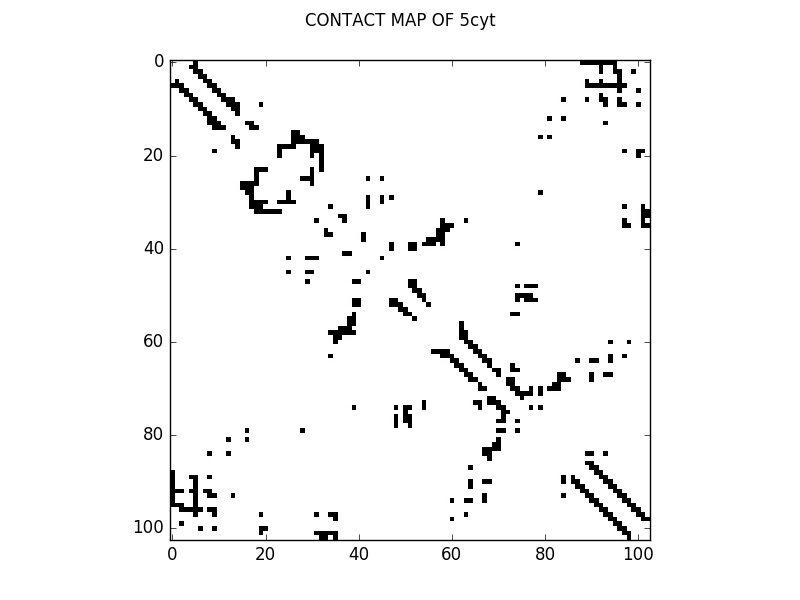
\includegraphics[width=0.8\textwidth]{figure4_contactmap_5cyt_c_CB.png}
\caption{Plot of classical contact map of a given residue}
\label{fig:ContactMap}
\end{figure}

\begin{figure}[h]
\centering
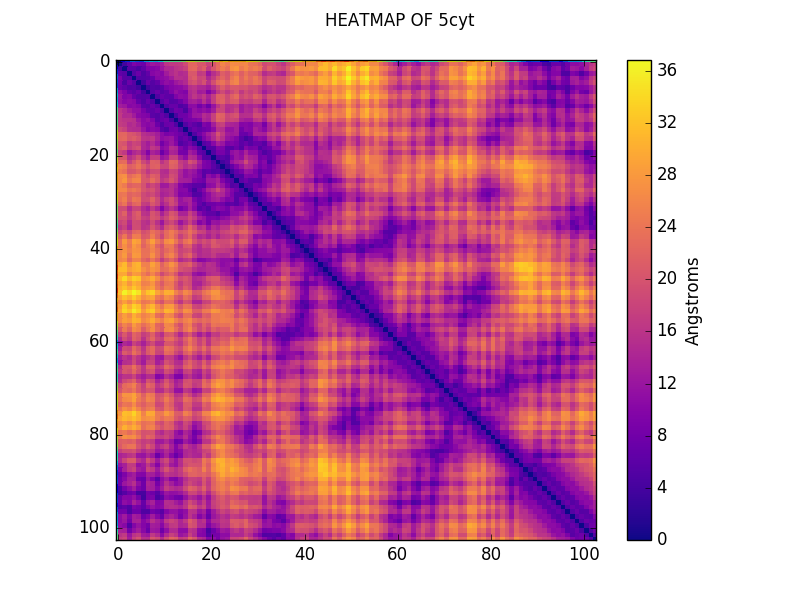
\includegraphics[width=0.8\textwidth]{figure5_heatmap_5cyt_d_CB.png}
\caption{Plot of heatmap of distances of a given residue}
\label{fig:HeatMap}
\end{figure}

\begin{figure}[h]
\centering
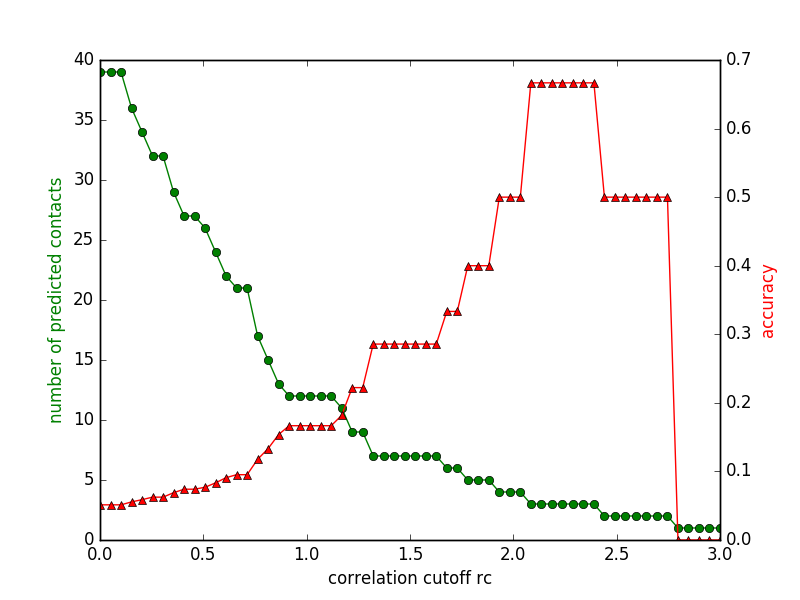
\includegraphics[width=0.8\textwidth]{figure6_accuracy_cutoffs_5cyt.png}
\caption{Accuracy, predicted contacts and correlation cutoff rc\cite{Gobel1994}.}
\label{fig:Accuracy}
\end{figure}

\begin{figure}[h]
\centering
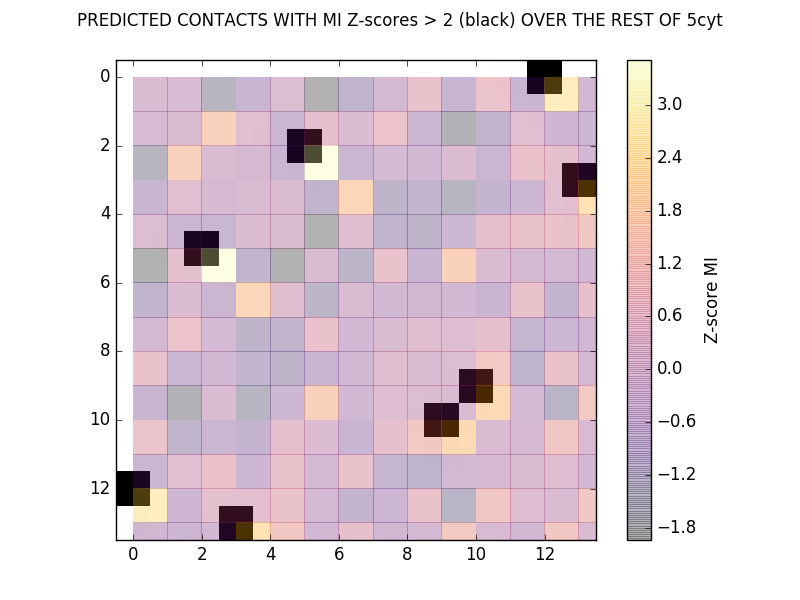
\includegraphics[width=0.8\textwidth]{figure2_supermatrix_5cyt_p_CB.png}
\caption{Predicted contacts with Z-score exceeding 2 over the rest of the Mutual Information Values}
\label{fig:Supermatrix}
\end{figure}

\begin{figure}[h]
\centering
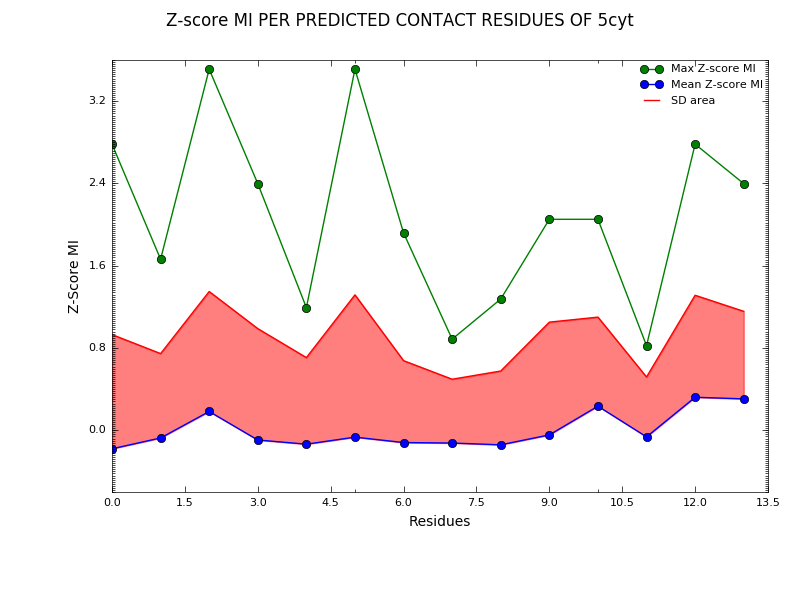
\includegraphics[width=0.8\textwidth]{figure1_Z-scoreMI_max_mean_5cyt_p_CB.png}
\caption{Parameters and plots MI z-score for predicted contacts per column vs residues}
\label{fig:MIZ}
\end{figure}

\subsection{Defining the contact map and distances heatmap for a protein}
First of all, for studying correlated mutations and distance correlation we need to assess all the possible contacts between residues inside of a protein. For that we need to study the contact map of a protein which is related to the distances between residues. As described in literature, the general tendency in describing distances between two residues is up to consider 8 \r{A} for $C_{\alpha}$ and $C_{\beta}$ as the minimum distance for consider that two residues are having contact . So, in order to study that, we decided to run our program for several proteins testing different distance thresholds being more restrictive or more permissive. The best results came when we apply 8 \r{A} as it has been described. In this way, the map of contact and also the plot of distances gives proof of it as contacts are describe in those points of the matrix that are below 8 \r{A}.\ref{fig:ContactMap} \ref{fig:HeatMap} \\

\subsubsection{Relating the contact map with the Mutual information for mutations in the sequence}
But are all the contacts described before equally informative in terms of mutational correlations? The answer is no. The contacts that need to be assessed are those that are informative in changes inside of protein sequence. As result of the extraction of sequences related with the one provided to our program we began to think if the type of multiple sequence alignment could have something important in assessing which are the residues important for correlated mutations and distances between residues. The answer to that question is that it doesn't matter. We get almost the same result using different strategies to perform MSA. So we thought that the bottle neck could be in the number of sequences provided among others facts. The truth is that it matters. For managing this in order to extract the best information possible we performed several test with different parameters. We calculated mutual information, selected with different mutual information cut-offs which are the most informative events and try to related them with their distances. Performing these trials we realized that the best mutual information cut-off was a value around 2 in the normalized score of mutual information or Z-score. Using that as a selection requirement we performed more test having promising results as described in the figure \ref{fig:Supermatrix}. \\

\subsection{Accuracy measurements of the predicted contacts}
As final part of our work, we needed to know if our program works properly and select actual informative events. For that we performed the dynamic of our precision and number of predicted contact for different cut-offs. We need to select where is the best condition for running such a test for our proteins. We decided to calculate the precision as it is described in bibliography (2016). We realized that for some proteins our programs cannot predict with high score of precision. But getting deeper in the field, we find out that the actual methods share the same luck as us. The maximum precision for several methods doesn't get higher than 0.5 and only one described method passed this value. Also we try to differentiate from so many others by searching a new vision of how our contacts behave. So we decided to study the differences between the most informative MI for each predicted contact and the average \ref{fig:MIZ}. The difference and also knowing that are more informative that the others can bring light on how these correlated mutations are behaving in our program. Evaluating how our program works we focus our effort in studying domains of single chain and small proteins of single chain, that are the best group that gave us the best results in terms of accuracy whereas if we test for larger proteins we have troubles having a good score \ref{fig:Accuracy}. That could be consequence of predicting contacts that are informative by randomness. So we get a lot of noise that we could not manage . \\


\clearpage
 \section{Conclusion}
Considering all the described before, it's clear that there is a long way in the improvement and understanding of correlated mutations and its relation with distance correlations and how significant are these two facts for protein residue co-evolution and its role in the 3D structure of proteins. New approaches like this one and so many others that are yet to come will have the word in making us closer to know preciselly how proteins changes can affect the function and stability of the structure of proteins. Beyond that, it is important to highlight that our vision and focus for this program at the level of small singled chained domains that are important in determining the function and features of several proteins can help us understand how nature is enough clever to preserve and maintain strategies among the evolution that are designed in a smart and reusable way. \\

However, limitations on the software are known to be improved and fulfilled successfully in order to tune up the perfomance of the program and making it usable for more types of PDB files. Such as PDB files containing multiple chains or just by adding a feature that allows the program to work also for protein-protein interactions. In the mean time, the program will help the study of domains by bringing information about what are the importanct residues that conserves the functionality and structure of the protein by their interactions with other residues. All this by helping us understanding more about co-evolution of residues in proteins. 


\clearpage
\listoffigures
\bibliography{tutorial}


\end{document}